\documentclass{sig-alternate}

\usepackage{amsmath,amssymb,amsfonts,amsmath}
\usepackage{hyperref}
\usepackage{color}
\usepackage{comment}
\usepackage{mdwlist}

\includecomment{mycomment}

%%%%%%%%%%%%%%%

\newcommand{\ff}[1]{\mathbb{F}_{#1}}
\newcommand{\fq}{\ff{q}}
\newcommand{\fqn}{\ff{q^n}}

\newcommand{\dd}{d}
\newcommand{\qq}{q}
\newcommand{\nn}{n}
\newcommand{\qn}{{\qq^\nn}}
\newcommand{\extfactfdegree}{k}
\newcommand{\extfactfsize}{\qq^{\nn \cdot \extfactfdegree}}

% if we define everything in terms of base field, extension field and
% extension field used in factorization
%
\newcommand{\basef}{\ff{\qq}}
\newcommand{\extf}{\ff{\qn}}
\newcommand{\extfactf}{\ff{\extfactfsize}}

\newcommand{\AG}{\mathrm{AG}(\qq,\nn)}

\DeclareMathOperator{\Tr}{Tr}
\DeclareMathOperator{\Ker}{Ker}
\DeclareMathOperator{\Ima}{Im} 
\DeclareMathOperator{\Decomp}{Decomp} 
\DeclareMathOperator{\Var}{Var} 
\DeclareMathOperator{\Exp}{E} 


% to specify the number of elements of the finite fields on which the
% trace is defined
\newcommand{\tr}[2]{\Tr_{\ff{#1}:\ff{#2}}}

% to specify the number of elements of the finite fields on which the
% trace is defined: light form
\newcommand{\trl}[2]{\Tr_{#1:#2}}

% to specify the notation of the finite fields on which the trace is
% defined
\newcommand{\trabs}[2]{\Tr_{#1:#2}}
\newcommand{\trextbase}{\trabs{\extf}{\basef}}
\newcommand{\trextfactext}{\trabs{\extfactf}{\extf}}
\newcommand{\trextfactbase}{\trabs{\extfactf}{\basef}}

\newcommand{\bigO}{O}
\newcommand{\bigOt}{\tilde{O}}
\newcommand{\smallO}{o}
\newcommand{\Mul}{\mathsf{M}}

\newcommand{\Span}{\mathbf{span}}
\newcommand{\card}[1]{\# #1}
\DeclareMathOperator{\Res}{Res}

\newcommand{\cost}[1]{\color{blue}Cost:  #1\color{black}}

%%%%%%%%%%%% Algorithms

\usepackage{float,algorithm}
\usepackage[noend]{algorithmic}
\renewcommand{\algorithmicrequire}{\textbf{Input:}}
\renewcommand{\algorithmicensure}{\textbf{Output:}}

\newcounter{algo}

\newenvironment{algorithm_noendline}[4]{\begin{center}\begin{minipage}{0.48\textwidth}
      \refstepcounter{algo}
      \label{#4}
      \sf
      \rule{\textwidth}{0.2pt}\\
      \makebox[\textwidth][c]{Algorithm~\arabic{algo}:~\textbf{#1}}\\
      \rule[0.5\baselineskip]{\textwidth}{0.2pt}\\

      \vspace{-12pt}

      \parbox{\textwidth}{\textbf{Input} #2}
      \parbox{\textwidth}{\textbf{Output} #3}

\vspace{-7pt}

      \begin{enumerate*}}{\end{enumerate*}
      \vspace{-11pt}
\end{minipage}\end{center}
}

\newenvironment{algorithm_endline}[4]{\begin{center}\begin{minipage}{0.48\textwidth}
      \refstepcounter{algo}
      \label{#4}
      \sf
      \rule{\textwidth}{0.2pt}\\
      \makebox[\textwidth][c]{Algorithm~\arabic{algo}:~\textbf{#1}}\\
      \rule[0.5\baselineskip]{\textwidth}{0.2pt}\\

      \vspace{-12pt}

      \parbox{\textwidth}{\textbf{Input} #2}
      \parbox{\textwidth}{\textbf{Output} #3}

\vspace{-7pt}

      \begin{enumerate*}}{\end{enumerate*}
      \vspace{-11pt}
      \rule{\textwidth}{0.2pt}
\end{minipage}\end{center}
%\vspace{-0.5cm}
}

\floatstyle{plain}
\newfloat{algofloat}{thp}{bla}
\floatname{algofloat}{}

%%%%%%%%%%

\newcommand{\todo}[1]{\textcolor{red}{TODO: #1}}
\newcommand{\com }{\noindent \textcolor{blue}{Commentaire Micha\"el}:}
\newcommand{\comd}{\noindent \textcolor{blue}{D\'ebut Micha\"el}:}
\newcommand{\comf}{\noindent \textcolor{blue}{:Fin Micha\"el}}




\newtheorem{Def}{Definition}
\newtheorem{Theo}{Theorem}
\newtheorem{Prop}{Proposition}
\newtheorem{Lem}{Lemma}
\newtheorem{Coro}{Corollary}

\renewcommand{\paragraph}[1]{\smallskip\noindent{{\bf \rm #1.}}}

\numberofauthors{3}
\author{
  \alignauthor Luca De Feo\\
  \affaddr{Laboratoire PRiSM}\\
  \affaddr{Universit\'e de Versailles}\\
  \email{luca.de-feo@uvsq.fr}
  \alignauthor Christophe Petit\\
  \affaddr{Crypto Group}\\
  \affaddr{University College London}\\
  \email{}
  \alignauthor Micha\"el Quisquater\\
  \affaddr{Laboratoire PRiSM}\\
  \affaddr{Universit\'e de Versailles}\\
  \email{mquis@prism.uvsq.fr}
}

\title{Deterministic root finding in small characteristic finite
  fields}

\begin{document}


\maketitle
\begin{abstract}
  The resolution of polynomial equations over finite fields has many
  applications, for example in cryptography or coding theory. Starting
  from the work of Berlekamp in the eighties, many efficient
  algorithms have been proposed to solve this problem faster, either
  asymptotically or in practice.  In this paper, we consider the case
  of polynomials over $\fqn$ where $\qq$ is a small number. We propose a
  new algorithm to solve this problem, merging features of Berlekamp's
  classical trace algorithm (BTA) and the recent successive resultant
  algorithm (SRA).  Similarly to BTA, our algorithm separates the
  roots of the polynomial into distinct subspaces using gcd
  computations. Similarly to SRA, it uses particular subspaces that
  are embedded in one another.

  Our algorithm has an asymptotic complexity similar to BTA and SRA on
  this type of polynomials ... It has this and this great advantages
  over these algorithms. Our Sage implementations show that it is
  great, easy to implement, very efficient, and beat previous
  algorithms on a large range of parameters...

  We also provide optimizations and a factorization version of our
  algorithm that are of further interest for SRA.
\end{abstract}

\category{F.2.1}{Theory of computation}{Analysis of algorithms and problem complexity}[Computations in finite fields]
\category{G.4}{Mathematics of computing}{Mathematical software}
\terms{Algorithms,Theory}
\keywords{Finite fields, root finding, factoring.}

%%%%%%%%%%%%%%%%%%%%%%%%%%%%%%%%%%%%%%%%%%%%%%%%%%%%%%%%%%%%
%%%%%%%%%%%%%%%%%%%%%%%%%%%%%%%%%%%%%%%%%%%%%%%%%%%%%%%%%%%%
%%%%%%%%%%%%%%%%%%%%%%%%%%%%%%%%%%%%%%%%%%%%%%%%%%%%%%%%%%%%

\section{Introduction}

This paper presents and compares two related algorithms for finding
roots of polynomials with coefficients in a finite field $\extf$,
where $\qq$ is small. The first algorithm, called the Successive
Resultants Algorithm (SRA), was already introduced by C.~Petit
in~\cite{cgUCL-P14}. We give here a fresh look at it and show how it
is related to the second one. The second algorithm, called the Affine
Refinement Method (ARM), is new, and similar in spirit to Berlekamp's
Trace Algorithm (BTA)~\cite{berl70}.

Both algorithms are deterministic. They find all the roots of a
square-free, split polynomial of degree $\dd$ using \todo{} operations
over $\basef$ in the worst case, and an expected \todo{} on
average. Hence, they improve over previously known deterministic
algorithms for root finding~\cite{Shoup91b} \todo{do they?}. For some
parameter ranges, they also compare favorably in practice with the
best randomized algorithms for root finding~\cite{berl70,cantor1981}.

Any algorithm for root finding can be extended to an algorithm for
factoring polynomials as mentioned in~\cite{Rabin79}. Doing so with
our algorithms does not improve over the previous literature
\todo{unless it does?}. However we argue in
Section~\ref{sec:factorization} that a partial application of this
idea yields a practical improvement to the classical Cantor-Zassenhaus
algorithm~\cite{cantor1981}.

\paragraph{Previous work} 

\paragraph{Our contribution}

\paragraph{Outline}


\section{Background and Notation}

We are interested in algorithms for the following problem: given a
degree $\dd$ polynomial $f(X)$ with coefficients in a finite field
$\extf$, find all the roots $\rho\in\extf$ such that $f(\rho)=0$.  

\paragraph{Complexity notations} In this paper, we use an
\emph{algebraic complexity model}, where the running time of an
algorithm is measured in terms of the number of operations ($+$,
$\times$, $\div$) in $\extf$, and its space requirements in terms of
number of elements of $\extf$ stored. As customary, we use the
$\bigO$-notation to neglect constant factors, and the
$\bigOt$-notation to further neglect poly-logarithmic factors. All
asymptotic complexities will be expressed in terms of the parameters
$\qq$, $\nn$ and $\dd$.

We denote by $\Mul : \mathbb{N} \to \mathbb{N}$ a function such that
polynomials in $\extf[X]$ of degree at most $m$ can be multiplied in
$\Mul(m)$ operations ($+$, $\times$) in $\extf$, and we make the
usual super-linearity assumptions on
$\Mul$~\cite[Chapter~8]{Gathen2003}.  Using FFT multiplication, we can
take $\Mul(m)\in\bigOt(m)$.


\subsection{Nested subspace decomposition of $\extf$}
\label{sec:nsd}

We now present the main ingredient of our algorithms. It consists in a
decomposition of the $\basef$-vector space $\extf$ into a sequence of
nested affine subspaces.

\paragraph{Approximating $\extf$ by a flag} Let
$\{\upsilon_1,\ldots,\upsilon_\nn\}$ be any basis of $\fqn/\fq$ (not
necessarily the one used to represent the elements of $\extf$). To
this basis, we associate the flag of linear subspaces $V_0\subset
V_1\subset \cdots \subset V_\nn$ defined by
\begin{equation}
  V_i = \Span(\upsilon_1,\dots,\upsilon_i),
\end{equation}
so that $\dim V_i = i$ and $\card V_i = \qq^i$. To each of the
subspaces we associate its minimal polynomial, that we denote by
$L_i$. Then we have the well know relation (see
\cite[Lemma~1]{cgUCL-P14})
\begin{equation}
  L_0(X) = X, \quad L_i(X) = (X^\qq - L_{i-1}(\upsilon_i)^{\qq-1}X)\circ L_{i-1}(X),
\end{equation}
where we remark that the $L_i$'s are linearized polynomials (see
\cite[Ch. 11]{Berlekamp1984}), and in particular $L_\nn=X^\qn-X$.

Notice that, by definition, each $L_i$ defines a linear map
$\extf\to\extf$, with kernel $V_i$. It will be convenient to encode
this information in an $\nn\times\nn$ matrix, thus we define
$\gamma_{i,j}=L_i(\upsilon_j)$, and
\begin{equation}
  \label{eq:Gamma}
  \Gamma =
  \begin{pmatrix}
    \gamma_{0,1} & \cdots & \gamma_{0,\nn}\\
    \vdots & & \vdots\\
    \gamma_{\nn-1,1} & \cdots & \gamma_{\nn-1,\nn}
  \end{pmatrix}.
\end{equation}
Observe that by definition $\gamma_{i,j}=0$ whenever $j\le i$, hence
$\Gamma$ is an upper triangular matrix, associated to a linear map
$\extf\to\extf^\nn$ sending any $\delta\in\extf$ to the vector
$L_0(\delta),\dots,L_{n-1}(\delta)$.  
\comd
 Il doit manquer un last quelque part.
\comf
We finally define $V_i^\ast$ as
the image space of $L_i$, i.e. the subspace generated by the $i$-th
row of $\Gamma$.  It is easily verified that $\dim V_i^\ast=n-i$ and
that $\{\gamma_{i,i+1},\dots,\gamma_{i,\nn}\}$ is a basis.

\comd
Let us define the dual of $L_i$, denoted by $L_i^\ast$, as the unique linearized polynomial (see
\cite[Ch. 11]{Berlekamp1984}) such that 
$$(L_i^\ast \circ L_i)(X)=(L_i^\ast \circ L_i)(X)=X^\qn-X\,.$$
In particular, $L_i^\ast(L_i(\alpha))=0$ for any $\delta \in \extf$. Therefore, $V_i^\ast=\Ker L_i^\ast=\Ima~L_i$.
\comf


\begin{Lem}
  The coefficients of the matrix $\Gamma$ can be computed using
  $O(\nn^2\log\qq)$ operations over $\extf$.
\end{Lem}
\begin{proof}
  By the recursive definition of $L_i$, it is clear that
  \begin{equation}
    \gamma_{i,j} =
    \begin{cases}
      \upsilon_j &\text{for $i=0$},\\
      \gamma_{i-1,j}^\qq - \gamma_{i-1,i}^{\qq-1}\gamma_{i-1,j} &\text{for $i>0$}.
    \end{cases}
  \end{equation}
  Thus, each $\gamma_{i,j}$ can be computed from the previous ones
  using $O(\log\qq)$ operations, and there is a total $O(\nn^2)$ of
  them to compute.
\end{proof}

The eigenvalues of $\Gamma$ play a special role in our algorithms,
thus we define $\beta_i=\gamma_{i-1,i}$ and $\alpha_i=\beta_i^{\qq-1}$
for any $1\le i \le \nn$. We deduce a decomposition
\begin{equation}
  X^\qn - X = (X^\qq - \alpha_\nn X) \circ \cdots \circ (X^\qq - \alpha_1 X).
\end{equation}

\paragraph{Covers of $\extf$ by affine subspaces} We now build a
sequence of covers of $\extf$ by affine subspaces, each one being a
subcover of the next one.

Let now $\rho\in\extf$, such that $\rho=\sum_jr_j\upsilon_j$.  For any
$V_i$ we define the affine space
\begin{equation}
  V_{i,\rho} = V_i + \rho.
\end{equation}
We also define the polynomial $M_{i,\rho}$ as the minimal polynomial
of $V_{i,\rho}$, hence
\begin{equation}
\label{node_product}
  M_{i,\rho}(X) = L_i(X - \rho) = L_i(X) - \sum_{j>i}r_j\gamma_{i,j}.
\end{equation}
Observe that $M_{i,\rho}=M_{i,\rho'}$, and thus
$V_{i,\rho}=V_{i,\rho'}$, if and only if $\rho-\rho'\in V_i$. Hence
there are exactly $\qq^{n-i}$ distinct affine spaces of the form
$V_{i,\rho}$, each of size $\qq^i$.

By definition we have
\begin{equation}
  V_{i,\rho} = \bigcup_{c\in\basef} V_{i-1,\rho + c\upsilon_i},
\end{equation}
hence
\begin{equation}
  M_{i,\rho}(X) = \prod_{c\in\basef} M_{i-1,\rho+c\upsilon_i}(X).
\end{equation}
Thus for each $i$, the distinct $V_{i,\rho}$'s form a cover of
$\extf$, and the $V_{i-1,\rho}$'s form a subcover of the $V_{i,\rho}$,
with $V_{i-1,\rho}\subset V_{i,\rho'}$ if and only if $\rho-\rho'\in
V_{i-1}$.  We deduce a sequence of factorizations of $X^\qn-X$ as
follows
\begin{equation}
  \label{eq:product-tree}
  \begin{gathered}
    X^\qn-X = M_{n,0}(X) =
    \prod_{c_1\in\basef}M_{n-1,c_1\upsilon_n}(X)=\\
    \prod_{c_1,c_2\in\basef}M_{n-2,c_2\upsilon_{n-1}+c_1\upsilon_n}(X)=\\
    \cdots=\\
    \prod_{c_1,\dots,c_n\in\basef}M_{0,c_n\upsilon_1+\cdots+c_1\upsilon_n}(X)=
    \prod_{\rho\in\extf}(X-\rho),
  \end{gathered}
\end{equation}
where the last equality comes from the fact that $L_0$ is the identity
map.

\comd
Let us finally remind some well-known facts about resultants.
Consider the polynomial $f \in \extf[X]$ and the projections $P_1, P_2 \in  \extf[X]$ and define $P$ as $P_2 \circ P_1$.
According to the property about the root's of resultants,
$$g(Y)=\Res_X(P(X)-Y,f(X))=\prod_{\{\rho \mid f(\rho)=0\}} (Y-P(\rho)) \,.$$
Therefore, the roots of the resultant $g(Y)$ are the projection of the roots of $f(X)$ throught $P$.
Also, 
\begin{equation}
\label{resultant_compose}
g(Y)=\Res_{Y_1}(L_2(Y_1)-Y,g^{(1)}(Y_1))
\end{equation}
 where $g^{(1)}(Y_1)=\Res_{Y_1}(L_1(X)-Y_1,f(X))$. Finally, 
 the algebraic multiplicity of a root of $g$ is the number of roots of $f$ projected to this root.
\comf


\section{Preliminaries}

In this section we review the fundamental subroutines upon which are
going to be based the algorithms of the next sections.

\todo{Do we need to remind the costs of:
  \begin{itemize}
  \item gcd?
  \item square-free factorization?
  \item ddf?
  \item modular composition?
  \item iterated frobenius and similar tricks?
  \item multipoint evaluation / interpolation?
  \end{itemize}
}

\begin{algorithm}
  \caption{Polynomial evaluation at special points}
  \label{alg:multi-ev}
  \begin{algorithmic}[1]
    \REQUIRE A polynomial $f\in\extf[X]$ of degree $\dd$,\\
    $\delta_0,\dots,\delta_\dd\in\extf$ and $\beta\in\extf$.
    \ENSURE $f(\delta_i+c\beta)$ for all $0\le i \le \dd$ and $c\in\basef$.
    \STATE Let $\alpha = \beta^{\qq-1}$;
    \STATE\label{alg:multi-ev:mod} Compute $\bar{f}(X,Y) = f \mod X^\qq-\alpha X-Y$;
    \STATE Let $\bar{f}(X,Y) = \sum_j \bar{f}_j(Y)X^j$;
    \STATE\label{alg:multi-ev:Delta} Compute $\Delta_i=\delta_i^\qq-\alpha\delta_i$ for $0\le i\le\dd$;
    \FOR {$0\le j<\qq$}
    \STATE\label{alg:multi-ev:multi-ev} Compute $\eta_{i,j}=\bar{f}_j(\Delta_i)$ for $0\le i\le\dd$;
    \ENDFOR
    \STATE Let $f_i(X) = \sum_j \eta_{i,j}X^j=\bar{f}(X,\Delta_i)$;
    \FOR {$0\le i \le\dd$}
    \STATE\label{alg:multi-ev:final-ev} Compute $\varepsilon_{i,c}=f_i(\delta_i+c\beta)$ for all $c\in\basef$;
    \ENDFOR
    \RETURN $\varepsilon_{i,c}$ for $0\le i\le\dd$ and $c\in\basef$.
  \end{algorithmic}
\end{algorithm}

\begin{Lem}
  \label{lem:multi-ev}
  Algorithm \ref{alg:multi-ev} is correct. On input a polynomial of
  degree $\dd\gg\qq$ and $O(\dd)$ evaluation points, it computes its
  output using $O(\Mul(\dd) \log\dd + \qq^2\Mul(\dd/\qq)\log\dd +
  \qq^2\dd)$ operations over $\extf$.
\end{Lem}
\begin{proof}
  Observe that
  $\prod_{c\in\basef}(X-\delta_i-c\beta)=X^\qq-\alpha X-\Delta_i$, with
  $\Delta_i$ defined as in step~\ref{alg:multi-ev:Delta}. Hence
  \begin{equation*}
    f_i(X)=f(X)\mod \prod_{c\in\basef}(X-\delta_i-c\beta)
  \end{equation*}
  Correctness follows immediately.

  We now analyze the complexity. In step~\ref{alg:multi-ev:mod}, we
  reduce $f$ so that $\bar{f}$ has degree $<\qq$ in $X$. This
  reduction can be computed in $O(\Mul(d)\log d)$ using a
  divide-and-conquer approach.

  By construction, the polynomials $\bar{f}_j(Y)$ have degree
  $O(\dd/\qq)$, hence step~\ref{alg:multi-ev:multi-ev} can be computed
  in $O(\qq\Mul(\dd/\qq)\log\dd)$ splitting the points $\Delta_i$ in
  $q$ batches, and using $\qq$ classical multi-point
  evaluations. Hence, the overall cost of the for loop is
  $O(\qq^2\Mul(\dd/\qq)\log\dd)$.

  Finally, step~\ref{alg:multi-ev:final-ev} can be computed again by
  multipoint evaluation in degree $O(\qq)$. However, we assume that
  $\qq$ is too small, to apply an asymptotically fast algorithm, thus
  we account $O(\qq^2)$ operations for this step, giving $O(\qq^2\dd)$
  operations for the whole loop. All other steps have negligible cost.
\end{proof}

\begin{algorithm}
  \caption{Resultant with a special polynomial}
  \label{alg:resultant}
  \begin{algorithmic}[1]
    \REQUIRE A polynomial $f\in\extf[X]$ of degree $\dd<\qq^{n-1}$,\\
    an element $\beta\in\extf$.
    \ENSURE The resultant $\Res_X\bigl(X^\qq-\beta^{\qq-1}X-Y,f(X)).$
    \STATE Let $\alpha=\beta^{\qq-1}$,
    \STATE\label{alg:resultant:select} Select points $\delta_0,\dots,\delta_d$ s.t. all $\delta_i^\qq-\alpha\delta_i$ are distinct;
    \STATE\label{alg:resultant:multi-ev} Compute $\varepsilon_{i,c}=f(\delta_i+c\beta)$ for $0\le i\le\dd$ and $c\in\basef$;
    \RETURN\label{alg:resultant:interp} $g$ such that $g\left(\prod_c\delta_i+c\beta\right) = (-1)^{\qq\dd}  \prod_c\varepsilon_{i,c}$.
  \end{algorithmic}
\end{algorithm}


\begin{Lem}
  \label{lem:alg-resultant}
  Algorithm~\ref{alg:resultant} is correct. On input a polynomial of
  degree $d\ll\qq^{\nn-1}$, it computes its output using $O(\Mul(\dd)
  \log\dd + \qq^2\Mul(\dd/\qq)\log\dd + \qq^2\dd)$ operations over
  $\extf$.
\end{Lem}
\begin{proof}
  It is well known that the resultant commutes with evaluation, i.e., if
  \begin{equation}
    g(Y) = \Res_X\bigl(X^\qq-\beta^{\qq-1}X-Y,f(X),\bigr),
  \end{equation}
  then
  \begin{equation}
    g(\Delta) = \Res_X\bigl(X^\qq - \beta^{\qq-1}X -\Delta , f(X)\bigr),
  \end{equation}
  for any $\Delta\in\extf$. Our algorithm is just a specialization of
  the classical evaluation-interpolation approach to compute bivariate
  resultants. We know that the polynomial $g$ has degree $\dd$, thus
  we only need to evaluate at $d+1$ points.

 % To make things simpler, we start by changing the sign of the right
  %operand, setting
  %\begin{equation}
  %  h(Y) = \Res_X\bigl(X^\qq-\beta^{\qq-1}X-Y, f(X)\bigr) = (-1)^\dd g(Y).
  %\end{equation}
  Let now $\delta\in\extf$ be such that
  $\Delta=\delta^\qq-\beta^{\qq-1}\delta$. By linearity we have
  \begin{multline}
    \label{eq:lin-resultant}
    \Res_X\bigl(X^\qq-\beta^{\qq-1}X-\Delta,f(X)\bigr) =\\
    \Res_X\Bigl(  \prod_{c\in\extf}(X-\delta - c\beta),f(X) \Bigr) =\\
    \prod_{c\in\extf} \Res_X\bigl(X-\delta - c\beta, f(X)\bigr) =\\
    (-1)^{\qq\dd} \prod_{c\in\extf} f(\delta+c\beta),
  \end{multline}
  where the second and third equalities comes from the
  multiplicativity of the resultant. The correctness of the algorithm
  now follows immediately.

  We now go to the complexity. The interpolation points at
  step~\ref{alg:resultant:select} can be selected at random, keeping
  track of the values $\Delta_i=\delta_i^\qq-\beta^{\qq-1}\delta_i$,
  and discarding duplicates. If $\dd\ll\qq^{n+1}$, we are likely to
  find enough points in $O(d)$
  tries. Step~\ref{alg:resultant:multi-ev} is computed using
  Algorithm~\ref{alg:multi-ev}, at the cost given in
  Lemma~\ref{lem:multi-ev}. Finally, step~\ref{alg:resultant:interp}
  is computed using a classical fast interpolation algorithm, at a
  cost $O(\Mul(d)\log d)$.
\end{proof}

Observe that the condition in Algorithm~\ref{alg:resultant} of having
$\dd+1$ points $\delta_i$ such that
$\Delta_i=\delta_i^\qq-\beta^{\qq-1}\delta_i$ are all distinct can
only be verified if $\dd+1\le\qq^{\nn-1}$. If more interpolation
points are needed, Eq.~\eqref{eq:lin-resultant} cannot be applied
anymore, but the evaluation-interpolation approach is still possible
at a slightly worse cost. However, this is not a major concern for the
algorithms we present next.



\section{The algorithms ARM and SRA}
\label{sec:arm-sra}

In this section we present two root finding algorithms based on the
structure of the affine space $\AG$. We start with the Affine
Refinement Method (ARM) of Menezes, van Oorschot and
Vanstone~\cite{Menvanovans92}, then go to the Successive Resultants
Algorithm (SRA) of Petit~\cite{cgUCL-P14}. For both, we present
variants which are more efficient than the original ones. Our
presentation highlights a link between the two algorithms that had
previously gone unnoticed: in both an abstract and a computational
sense, ARM and SRA can be seen as \emph{dual} to each other.

ARM works by \emph{intersecting} the roots of the input polynomial
with the subspaces $V_{i,\rho}$. The successive intersections are
computed by means of GCDs.  SRA works by \emph{projecting} the roots
onto the spaces $V_i^\ast$.  The successive projections are computed
by means of resultants.

At an algorithmic level, the duality is embodied in the well known
property
\begin{equation}
  \gcd\bigl(f(X),g(X)\bigr) \ne 1 \;\Leftrightarrow\; \Res_X\bigl(f(X),g(X)\bigr)=0\,,
\end{equation}
which implies that ARM isolates a root of $f$ whenever SRA does.

\paragraph{Pre-computation} Both methods take as input a basis
$\upsilon_1\dots,\upsilon_\nn$, and use it to define the affine space
$\AG$ as in Section~\ref{sec:nsd}. To this end, they compute the
matrix $\Gamma$ of Eq.~\eqref{eq:Gamma} at a cost of $O(n^2\log q)$
operations. Note that this phase depends only on the field and may be
re-used for the root-finding of several polynomials defined on the
same field.

\paragraph{ARM} The method consists in \emph{intersecting} the roots of $f$ with the corresponding fibers of $L_i$ identified by $\ell_i \in V_i^\ast$.
%The method consists in \emph{projecting} the roots of $f$ onto the spaces $V_i^\ast$ while simultaneously \emph{intersecting} those with the corresponding fibers of $L_i$ identified by $\ell_i$.
 It is achieved by computing the non-constant gcd's among the set
% the computation of the minimal polynomial of those intersections by means of gcd's, i.e. 
 \begin{equation}
 \label{base_ARM}
\gcd(L_i(X)-\ell_{i,\rho},f(X))     \mbox{ with }  \ell_{i,\rho}  \in V_i^\ast\,,
\end{equation}
for $i$ starting from $n$ and going down to 0.
It ultimately leads to the root of $f$ because 
$$\gcd(L_0(X)-\ell_{0,\rho},f(X))=\gcd(X-\ell_{0,\rho},f(X)) \ne 1\,,$$ 
provide the linear factors of $f$. 
Note that 
\begin{equation}
  \label{eq:duality-gcd}
  \gcd(L_i(X)-\ell_{i,\rho},f(X)) \ne 1
\end{equation}
means that there is a root of $f$ in the fiber $\{\rho' \mid L_i(\rho')=\ell_{i,\rho} \}$.
In practice, these gcd's are computed in a recursive way. Let us first define
 $$f_{i,\rho}(X)=\gcd(L_i(X)-L_i(\rho),f(X))\,$$
where $\rho \in \extf$. Hence $f_{i,\rho}(X)=f_{i,\rho'}(X)$ if and only if $\rho-\rho' \in V_i$.
Using Eq.~\eqref{base_ARM} and the fact that $V_n^\ast=\{0\}$, $f_{n,0}(X)$ is first computed, i.e.,
 $$f_{n,0}(X)=\gcd(L_n(X),f(X))=\gcd(X^{q^\nn}-X,f(X))\,.$$
The recursive step is based on Eq.~\eqref{node_product} and works as follows: for any $L_i(\rho) \in V_i^\ast$ such that $f_{i,\rho}(X)$ is neither a constant polynomial nor a linear factor,
  $$
  \begin{array}{lll}
  f_{i,\rho}(X)&=&\prod_{c \in \basef} \gcd(M_{i-1,\rho+c \cdot \upsilon_i}(X),f_{i,\rho}(X)) \\
               &=&\prod_{c \in \basef} \gcd(L_{i-1}(X)-L_{i-1}(\rho+c \cdot \upsilon_i),f_{i,\rho}(X)) \\
               &=&\prod_{c \in \basef} f_{i-1,\rho+c \cdot  \upsilon_i}(X)\\
  \end{array}              
  $$ 
 
 This procedure builds a tree where at each level only the nodes containing a polynomial of degree strictly greater than 1 are branched. Said otherwise, the leafs of the tree are either constant polynomials or the distinct linear factors of $f$ (without their algebraic multiplicity). ARM is summarized in Algorithm~\ref{alg:arm}.

%Note that the $l_i$ for which $\gcd(f(X),L_i(X)-l_i) \ne 1$ correspond to the $L_i$-projections onto $V_i^\ast$ of the roots of $f$.
  
 \begin{algorithm}
   \caption{Affine Refinement Method}
   \label{alg:arm}
   \begin{algorithmic}[1]
   \REQUIRE {A polynomial $f\in\extf[X]$ of degree $\dd$,\\
     A basis $\upsilon_1,\dots,\upsilon_\nn$ of $\extf$,\\
     The matrix $\Gamma=(\gamma_{i,j})$ defined in~\eqref{eq:Gamma}.}
   \ENSURE {The roots of $f$ in $\extf$.}
   \STATE Set $L_0 = X$;
   \FOR {$1 \le i \le \nn$}
   \STATE\label{alg:arm:Li} Compute $L_i = L_{i-1}^\qq - \gamma_{i-1,i}^{\qq-1} L_{i-1} \mod f$;
   \ENDFOR
   \STATE Initialize tree with root $f_{\nn,0} = f \mod L_\nn$;
   \FOR {$\nn \ge i \ge 1$}\label{alg:arm:for}
   \FOR {any node $f_{k,\rho}$ of degree $>1$ in the tree}
   \STATE\label{alg:arm:combili} Compute $\ell_{i-1,\rho} = L_{i-1}(\rho) = \sum_j r_j\gamma_{i-1,j}$;
   \ENDFOR
   \FOR {any leaf in the tree $f_{i,\rho}$ of degree $>1$}
   \STATE\label{alg:arm:mod} Compute $\bar{L}_\rho = L_{i-1}\mod f_{i,\rho}$;
   \FOR {any $c\in\basef$}
   \STATE\label{alg:arm:gcd} $f_{i-1,\rho+c\cdot \upsilon_i} = \gcd(\bar{L}_\rho - \ell_{i-1,\rho} - c\gamma_{i-1,i}, f_{i,\rho})$;
   \ENDFOR
   \ENDFOR
   \IF {all leaves have degree $\le 1$}
   \RETURN The root of each leaf of degree $1$.
   \ENDIF
   \ENDFOR
   \end{algorithmic}
 \end{algorithm}

 \begin{Lem}
   Algorithm~\ref{alg:arm} (ARM) is correct. If the root tree for the
   input $f$ and $\upsilon_1,\dots,\upsilon_\nn$ has depth $h$, it
   computes its output using $O(\nn\Mul(\dd)\log\qq + h^2\dd +
   h\qq\Mul(\dd)\log\dd)$ operations over $\extf$.
 \end{Lem}
 \begin{proof}
   Correctness has been discussed above. Concerning complexity, the
   computation of the polynomials $L_i$ in step~\ref{alg:arm:Li} is
   done in $O(\Mul(\dd)\log\qq)$ for each polynomial, contributing
   $O(\nn\Mul(\dd)\log\qq)$ to the total.

   Now we treat the steps inside loop~\ref{alg:arm:for}.  Each of the
   complexities below is multiplied by $h$ in the total count.

   In step~\ref{alg:arm:combili}, we need to compute $L_{i-1}(\rho)$
   for each root approximation $\rho$ in the tree. If $\rho$ is the
   approximation associated to a node, and $\rho'$ is the
   approximation associated to its parent, then
   $\rho-\rho'=c\upsilon_j$ for some $c\in\basef$ and some basis
   vector $\upsilon_j$. Hence, knowing the elements $\gamma_{i-1,j}$,
   the value $L_{i-1}(\rho)$ can be computed from $L_{i-1}(\rho')$
   using only one field operation. At any iteration, there are at most
   $hd$ nodes in the tree, hence a cost of $O(hd)$.

   Step~\ref{alg:arm:mod} can be computed putting all $f_{i,\rho}$
   together in a subproduct tree, as in the classical multi-point
   evaluation algorithm. Reducing modulo the subproduct tree costs
   then $O(\Mul(\dd)\log\dd)$.

   Finally, in step~\ref{alg:arm:gcd} the degrees of the polynomials
   $f_{i,\rho}$ sum up to $\dd$. For each of these, we compute $\qq$
   gcd's with polynomials of similar degree. Each of these polynomials
   can be computed in $O(\Mul(\dd_\rho)\log\dd_\rho)$, where
   $\dd_\rho$ is the degree of $f_{i,\rho}$. Summing over all
   polynomials, and using the super-linearity of the function $\Mul$,
   we bound this by $O(\qq\Mul(d)\log d)$.
 \end{proof}

\paragraph{SRA} The method consists in \emph{projecting} the roots of $f$ onto the spaces $V_i^\ast$ for $i$ starting from $n$ and going down to 0.
It is achieved by the computation of the values $\ell_{i,\rho} \in V_i^\ast$ annihilating
 \begin{equation}
 \label{base_SRA}
\Res_X(L_i(X)-\ell_{i,\rho},f(X)) \,.
\end{equation}
It ultimately leads to the roots of $f$ because
$$\Res_X(L_0(X)-\ell_{0,\rho},f(X))=\Res_X(X-\ell_{0,\rho},f(X))=0\,$$
means that $\ell_{0,\rho}$ is a root of $f$. Note that 
\begin{equation}
  \label{eq:duality-res}
  \Res_X(L_i(X)-\ell_{i,\rho},f(X)) =0
\end{equation}
means that there is a root of $f$ in the fiber $\{\rho' \mid
L_i(\rho')=\ell_{i,\rho} \}$.  Comparing this with
Eq.~(\ref{eq:duality-gcd}), the duality between ARM and SRA becomes
apparent. Indeed, $\gcd(L_i(X)-\ell_{i,\rho},f(X)) \ne 1$ if and only
if $\Res_X(L_i(X)-\ell_{i,\rho},f(X)) =0$.

Like ARM, SRA is a two-swipes algorithm.  We first compute the
polynomials $f^{(i)}$ having as roots the projections onto $V_i^\ast$
of the roots of $f$, i.e.,
$$f^{(i)}(Y_i)=\Res_{X}(L_i(X)-Y_i,f(X))  \mbox{ for }i=0 \cdots n \,.$$
The polynomial $f^{(i)}$ is computed from $f^{(i-1)}$ by projecting
its roots onto $V_i^\ast$. By the definition of $L_i$, we have  $f ^{(0)}=f$ and
$$f^{(i)}(Y_i)=\Res_{X_{i-1}}(X^q_{i-1} - \alpha_i X_{i-1} -Y_i,f^{(i-1)}(X_{i-1})) \,.$$

At each iteration, some roots of $f^{(i-1)}$ may be projected to the
same root of $f^{(i)}$. We apply a square-free factorization algorithm
to only keep one representative of those roots. Doing this allows us
to stop the descent before $f^{(n)}$ is computed. Indeed, we can
verify that $f^{(i)}=L_i^\ast$ simply by checking the degree of
$f^{(i)}$, then we know that the roots of $f^{(i)}$ are all the
elements of $V_i^\ast$. In the worst case, this will happen at the
last step, when $f^{(n)}(X)=X=L_n^\ast(X)$, and the only root is $0$.
In practice, the square-free factorization is unlikely to
significantly reduce the degree of $f$ before the last $\log\dd$
iterations, it is thus advisable to skip it in the first ones.

After the $f^{(i)}$'s are computed, SRA iteratively computes their
roots starting from the last. The roots of $f^{(i-1)}$ are deduced
from those of $f^{(i)}$ using Eq.~\eqref{Li_generation}. For any root
$\ell_i$ of $g^{(i)}$ belonging to $V_i^\ast$, we check whether
$g^{(i-1)}(\ell_{i-1})=0$ for any $\ell_{i-1} \in V_{i-1}^\ast$ such that
$\ell_{i-1}^\qq-\alpha_i \cdot \ell_{i-1}=\ell_i$. This procedure builds
a tree where at level $i$ the nodes are the roots of $g^{(i)}$.  The
leafs of the tree at level $0$ are the roots of $f$.

  
 \begin{algorithm}
   \caption{Successive Resultant Algorithm}
   \label{alg:sra}
   \begin{algorithmic}[1]
   \REQUIRE {A polynomial $f\in\extf[X]$ of degree $d$,\\
     A basis $\upsilon_1,\dots,\upsilon_\nn$ of $\extf$,\\
     The matrix $\Gamma=(\gamma_{i,j})$ defined in~\eqref{eq:Gamma}.}
   \ENSURE {The roots of $f$ in $\extf$.}
   \STATE Let $f^{(0)}=f$;
   \FOR {$1\le i \le \nn$}\label{alg:sra:for1}
   \STATE\label{alg:sra:resultant} $\hat{f}^{(i)}(Y) = \Res_X(X^\qq - \gamma_{i-1,i}^{\qq-1}X-Y,f^{(i-1)}(X))$;
   \STATE\label{alg:sra:sqfree} Compute $f^{(i)}$, the square-free part of $\hat{f}^{(i)}$;
   \IF {$\deg f^{(i)} = \qq^{\nn-i}$}
   \STATE Set $h=i$;
   \STATE {\bf break} out of the {\bf for} loop;
   \ENDIF
   \ENDFOR
   \STATE Let $A_h = (\rho_0,\dots,\rho_{\qq^{\nn-h}})$ such that $V^\ast_h=\bigl(L_h(\rho_j)\bigr)_j$;
   \FOR {$h> i\ge 0$}\label{alg:sra:for2}
   \FOR {any $\rho\in A_i$}
   \STATE\label{alg:sra:combili} Compute $\ell_{i,\rho}=L_i(\rho)=\sum_jr_j\gamma_{i,j}$;
   \ENDFOR
   \STATE\label{alg:sra:eval} $E_i = \left(f^{(i)}(\ell_{i,\rho} + c\gamma_{i,i+1}) \text{ for any $\rho\in A_{i+1}$ and $c\in\basef$}\right)$;
   \FOR {any $\rho\in A_i$}
   \STATE Add $\rho+c\upsilon_{i+1}$ to $A_i$ only if $f^{(i)}(\rho+c\gamma_{i,i+1})=0$.
   \ENDFOR
   \ENDFOR
   \RETURN $A_0$.
   \end{algorithmic}
 \end{algorithm}

 \begin{Lem}
   Algorithm~\ref{alg:sra} (SRA) is correct. If the root tree for the
   input $f$ and $\upsilon_1,\dots,\upsilon_\nn$ has depth $h$, it computes its
   output using $O\left(h(\Mul(\dd)\log \dd +
     \qq^2\Mul(\dd/\qq)\log\dd + \qq^2\dd + h\dd)\right)$ operations
   over $\extf$, or more compactly $O(h\qq\Mul(\dd)\log\dd + h^2\dd)$.
 \end{Lem}
 \begin{proof}
   Correctness has been discussed above. Concerning complexity, we
   remark that any step in loop~\ref{alg:sra:for1} and
   loop~\ref{alg:sra:for2} is repeated exactly $h$ times, thus the
   overall complexity is multiplied by $h$.

   Step~\ref{alg:sra:resultant} can be computed using
   Algorithm~\ref{alg:resultant}. According to
   Lemma~\ref{lem:alg-resultant}, this costs $O(\Mul(\dd) \log\dd +
   \qq^2\Mul(\dd/\qq)\log\dd + \qq^2\dd)$.

   Step~\ref{alg:sra:sqfree} is computed in $O(\Mul(\dd)\log\dd$ using
   a classical algorithm.

   The elements $L_i(\rho)$ in step~\ref{alg:sra:combili} are computed
   using the tree structure of the roots, like in ARM, thus requiring
   only one field operation per value. There are at most $hd$
   approximations at each iteration, thus this step contributes
   $O(hd)$ operations.
   
   Finally, step~\ref{alg:sra:eval} can be computed using the
   multi-point evaluation algorithm~\ref{alg:multi-ev}, at the same
   cost of step~\ref{alg:sra:resultant}.
 \end{proof}

 Using the two previous lemmas, we can now easily state the worst case
 complexity of both ARM and SRA, indeed for both algorithms the height
 $h$ equals $\nn$ in this case. Unsurprisingly, the two algorithms
 have very similar complexities.

 \begin{Theo}
   In the worst case, both ARM and SRA compute their output using
   $O(nq\Mul(d)\log d + n^2d)$.
 \end{Theo}
 
 On average, however, both algorithms will stop before reaching the
 bottom of the tree. The goal of the next section is to analyze the
 behavior of ARM and SRA on average.


\subsection{Expected number of iterations of ARM}

Define the operator which associate to each element of $\extf$ its $k$ last components in the basis $\{v_1, \cdots, v_n\}$, i.e. 
$$\pi_k:\extf \rightarrow \mathbb{F}_{\qq}^{k}: \rho=\sum_j r_j v_j \mapsto \pi_k(\rho)=(r_{n-k+1}, \cdots , r_n)\,.$$
Consider the $\qq$-ary tree were each node may be uniquely specified by $\pi_i(\rho)$ and contains $f_{n-i,\rho}$ the minimal polynomial of the distinct roots of $f$ belonging to $V_{n-i,\rho}$. The root of the tree is specified by $\emptyset$ and contains $f_{n,0}(X)=\gcd(X^{\qq^\nn} -X,f(X))$. If each branch from a node are labelled with a element of $\basef$, the components of $\pi_i(\rho)$ specify the path from the root to that node.

As already explained in section~\ref{ARM_SRA_description}, ARM algorithm consists essentially in building a subtree of the above tree.  Only nodes containing polynomials 
$f_{n-i,\rho}$ with degree strictly higher than 1 are branched. It means that leafs of this subtree contain either a constant polynomial or a linear factor of $f$ and may appear at whatever level. Observe that a leaf $\pi_i(\rho)$ containing a linear factor of $f$ is present in this subtree if and only if $V_{n-i,\rho}$ contains only one root of $f$ and $i$ minimal.
 The number of iteration $h$ of ARM is therefore the height of the subtree or equivalently the number of "digits", starting from the end, we need to consider to distinguish the roots $\rho=\sum_j r_j v_j$  of $f$. This height will depends on the way the roots of the polynomial $f$ are distributed among the $V_{i,\rho}$'s.
 
\medskip 
 
\noindent {\bf Worst case analysis:} As observed by Menezes, Van Oorschot and Vanstone~\ref{Menvanovans92}, the depth of the subtree of ARM will be maximal if $f$ contains two roots in some $V_{1,\rho}$. In this case, those two roots will be separated only at the $\nn^{th}$ iteration. Also, as observed by C. Petit~\ref{cgUCL-P14} the number of nodes of the subtree will be maximal, and so is the complexity of ARM (and SRA), if the roots of $f$ may be divided in pairs such that each of them belong to a distinct $V_{1,\rho}$. 
 
\medskip 

\noindent {\bf Statistical analysis:}
As already observed by Menezes, Van Oorschot and Vanstone~\ref{Menvanovans92}, this problem is highly related to the expected height of data structure called \emph{digital tries}. The match is nevertheless not complete and digital tries may be viewed as a limit object of our situation. Therefore, we discuss here relevance of the results on digital tries to our problem.

Let first remind what is a digital tries. It is a ordered tree data structure that is used to store a dynamic set or associative array where the keys are (possibly infinite) strings whose components belong to an alphabet $\mathcal{A}$ with $m$ elements. Therefore it is an $m-$ary tree with the property that nodes on level $l$ represent the set of all keys that begin with a certain sequence of $l$ characters called its \emph{prefix}. The root is associated with the empty string. The access path from the root to a leaf is minimal prefix of the key contained in the leaf. The height of a \emph{digital tries} is therefore the minimum number of digits required to distinguish the keys. Many authors studied the statistical behaviour of a digital tries, e.g.~\cite{szpankowski1986analysis} which depends on the way the keys are generated. The Bernoulli model is as follow:
\begin{enumerate}
\item A key $X_k=(x_{k1},x_{k2}, \cdots)$ is a sequence of elements (digits) from the alphabet $\mathcal{A}$ which form an independent sequences of Bernoulli trials with $P(x_{kj}=\alpha_i)=p_i$ for $k=1,\cdots, n$ and $i=1, \cdots, m$
\item The keys $X_1, \cdots, X_{\dd} $ are independent where $\dd$ is a fixed value.
\end{enumerate}
One of the main quantity of interest is the height $H_{\dd}$ of the a digital trie under the Bernoulli model. As proved in Szpankowski~\cite{szpankowski1986analysis}, if we define  $u^{-1}=\sum_{i} p_i^2$ we have:
\begin{enumerate}
\item $\Exp(H_{\dd}) \le 2 \log_m \dd +1 +\frac{1-ln~2}{ln~u} + \bigO(\dd^{-1})$,
\item $\lim\limits_{\dd \to \infty} P(H_\dd < x + 2 \cdot \log_u \dd)=exp(-exp(-x \cdot ln~u))$.
\end{enumerate}
From the second statement, Szpankowski~\cite{szpankowski1986analysis} derived that: 
\begin{enumerate}
\item $\Pr(H_\dd <x) \approx exp(-exp(-ln~u \cdot (x-2 \cdot \log_u \dd)))$
\item $\Var H_\dd \approx \frac{\pi^2}{6 \cdot (ln~u)^2}$
\end{enumerate}

\noindent {\bf Link between digital tries and our context:} The main difference between the two contexts is that the height of our tree is bounded by the degree of the field extension, denoted by $H'_\dd$, while the height of digital tries $H_\dd$ are only bounded by the number of keys they contain. If the roots of the root of the tree $f_{n,0}$ are uniformly chosen in $\extf$ and independently and assumed to be $\dd$, in this case the key are the roots of $f_{n,0}$ and it is not hard to see that $H'_\dd \le min(H_\dd,\nn)$. 
 Note that in practice, the roots of $f_{n,0}(X)=\gcd(X^{\qq^\nn} -X,f(X))$ are not chosen independently because the $\gcd$ guarantees that all the roots are different.

Analysing the statistical behavior of $H_\dd$ with the parameters $m=\qq$ and $p_i=\frac{1}{\qq}$ will allows to give bounds on indicators on  $H'_\dd$. We have that $u^{-1}=\sum_i (1/\qq)^2=1/\qq$. Therefore, $u=\qq$.
Assume that  the number of the roots is smaller than $\qq^{\frac{\nn}{2}}$, then the approximation on the independency is valid according to the birthday paradox and the we have $\Exp(H_\dd) \le 2 \log_\qq \dd +1 +\frac{1-ln~2}{ln~\qq} + \bigO(\dd^{-1})$. Therefore, for any $\dd \le \qq^\nn$
$$\Exp(H' _\dd) \le  min(2 \log_\qq \dd +1 +\frac{1-ln~2}{ln~\qq} + \bigO(\dd^{-1}), \nn)\,.$$
The two next results requires that we may approximate $H'_\dd$ by $H_\dd$ and in particular that independency holds. Therefore that $\dd \le \qq^{\frac{\nn}{2}}$
$$\Pr(H'_\dd <x) \approx exp(-exp(-ln~\qq \cdot (x-2 \cdot \log_\qq \dd)))\,.$$
and 
$$\Var H'_\dd \approx \frac{\pi^2}{6 \cdot (ln~\qq)^2}\,.$$
Those two results express the fact that generally, the algorithm won't escape very much from his average.


Finally, note that there is a typo in Menezes, Van Oorschot and Vanstone~\ref{Menvanovans92} on the the bound on the number of iterations which is stated as $ 2\log_q \nn + \bigO(1)$  instead of $2\log_q \dd + \bigO(1)$. This leads to typos in their complexity evaluation of the Affine method, ARM and BTA.




\section{Variant and Extensions}

\subsection{Decomposition of the field equation when $n$ is composite}

\noindent Both root-finding method, SRA and ARM, require first to write down the field equation as the composition of elementary linearized polynomials, i.e. $X^{q^n}-X=\circ_{i=1}^n (X^q-\alpha_i^{q-1} \cdot X)$.
As previously seen, the $\alpha_i$ can be computed in $\mathcal{O}(\log q \cdot n^2)$ operations in $\mathbb{F}_{q^n}$. When $n$ is composite, generic formula may be deduced 
which allows to decrease the time complexity of the computation.

\medskip   

\noindent It is well known that $(\mathbb{F}_q[X],\cdot)$ is isomorphic to  $(\mathbb{F}_q[\sigma], \circ)$, where $\sigma: X \mapsto X^q$ is the Frobenius map over $\mathbb{F}_{q^n}$  and $q$ is a prime power. 
Elements related by this isomorphism are said $q-$associated. 

\medskip

\noindent Consider now the case $n=p^i \cdot r$, where $p$ is the characteristic of $\mathbb{F}_q$ and $\gcd(r,p)=1$.  
The field equation $X^{q^{p^i \cdot r}}-X$ is $q$-associated to the polynomial $x^{r\cdot p^i}-1 \in \mathbb{F}_q[X]$. Also, according
 to the linearity of the Frobenius,  $x^{r \cdot p^i}-1=(x^r-1)^{p^i}$. Therefore 
$$X^{q^{p^i \cdot r}}-X=\circ^{p^i} (X^{q^r}-X)\,,$$
where $\circ^{k} P(X)$ means that $P(X)$ is composed $k$ times with itself. 

\medskip

\noindent In what follows, we consider w.l.o.g the decomposition of the field equation $X^{\qq^n}-X$ where $\gcd(n,p)=1$ and $p$ is the characteristic of the field. We first prove a technical lemma which will allow us to decompose field equation in different ways.

\medskip

According to theorem 3.68 of "Finite Fields"~\cite{LildNiderreiter}, any $\qq^m$-linearized polynomial $L'(X)$ over $\mathbb{F}^{\qq^{m \cdot s}}$ $L'(X)$ may be decomposed into $\qq^m$-linearized polynomials as $L'(X)=L_I(X) \circ L(X)$ where $L_I(X)$ has no root in $\mathbb{F}^{\qq^{m \cdot s}}$ and  $L(X)$ is the $\qq^m$-linearized minimal polynomial of $Ker~L'$. The next Lemma show how to decompose the $L(X)$ part.

\begin{Lem}
\label{linearized_decomposition}
Let $\{u_1, \cdots, u_r\}$ be a basis of a vector subspace of $\mathbb{F}_{\qq^{ms}}/\mathbb{F}_{\qq^m}$ and $L(X)$ be the
 $\qq^m$-linearized minimal polynomial over $\mathbb{F}_{\qq^{ms}}$ of this basis. Assume we know the decomposition
$X^{\qq^{m}}-X=\circ_{i=1}^{m} (X^{\qq}-(\beta_i')^{\qq-1} X)$ where $\beta_i' \in \mathbb{F}_{\qq^{m}}$. Then, $L(X)$ may be decomposed as
$$L(X)=\circ_{j=1}^{r} \left( \circ_{i=1}^{m} (X^\qq-(\beta_i'  \beta_j^{\qq^{i-1}})^{q-1}   X) \right)$$
where $\beta_j \in \mathbb{F}_{\qq^{m\cdot s}}$. Moreover, the $\beta_i$ and the cross-product $\beta_i' \beta_j^{q^{i-1}}$ may be computed in 
$$\bigO(\log q \cdot m \cdot r^2 \cdot \Mul(m \cdot s))$$
operations in $\basef$.
\end{Lem}
\begin{proof}
By hypothesis,  $\{u_1, \cdots, u_r\}$ is a basis of $\Ker L$ over $\mathbb{F}_{\qq^m}$.  To this basis, we associate the polynomials $K_j$ defined by $K_0(X)=X$ and 
$$K_{j+1}(X)=K_j(X)^{\qq^{m}}-K_j(u_{j+1})^{\qq^{m}-1} \cdot K_j(X)$$
 for $j=0, \cdots r-1$. Note that $K_r(X)=L(X)$ because they are both monic, $\Ker K_r=\Ker L$, they share the same degree and $L$ is minimal. Therefore,
$$L(X)=\circ_{j=1}^r (X^{\qq^m} -\beta_j^{\qq^m-1}X) $$
where $\beta_j=K_{j-1}(u_i) \in \mathbb{F}_{\qq^{ms}}$.
%(X^{\qq^m} -X $$
%\beta_j^{\qq^{m}-1}
Also,  
\begin{equation}
\label{basic_decomp}
(X^{\qq^{m}}-\beta_j^{\qq^{m}-1} X)= (\beta_j^{\qq^{m}} X) \circ (X^{\qq^{m}}-X)\circ(\beta_j^{-1}X)\,.
\end{equation}
By hypothesis $X^{\qq^{m}}-X$ may be decomposed as
\begin{equation}
\label{decomp_basef}
X^{\qq^{m}}-X=\circ_{i=1}^{m} (X^{\qq}-(\beta_i')^{\qq-1} X)\,,
\end{equation}
where $\beta_i' \in \mathbb{F}_{\qq^{m}}$. Therefore, substituting this decomposition in the previous equation, $(X^{\qq^{m}}-\beta_j^{\qq^{m}-1} X)$ reduces to 
$$(\beta_j^{\qq^{m}} X) \circ    \left(    \circ_{i=1}^{m} (X^{\qq}  -(\beta_i')^{\qq-1}    X)  \right) \circ(\beta_j^{-1}X)\,.$$
%It follows that $X^{\qq^\nn}-X$ decomposes as
%$$\circ_{j=1}^{n_2} \left(   (\beta_j^{\qq^{n_1}} X) \circ    \left(    \circ_{i=1}^{n_1} (X^{\qq}  -(\beta_i')^{\qq-1}    X)  \right) \circ(\beta_j^{-1}X)    \right) $$
This last expression may be written as
$$\circ_{i=1}^{m} \left( ((\beta_j^{\qq^{i-1}})^\qq X) \circ  (X^{\qq}- (\beta_i')^{\qq-1}    X) \circ   ((\beta_j^{\qq^{i-1}})^{-1}X)  \right)\,.$$ 
Noting that each expression in the above decomposition is simply $X^\qq-(  \beta_i'  \beta_j^{\qq^{i-1}})^{q-1}  X$, we have
\begin{equation}
\label{decomp_partial}
(X^{\qq^{m}}- \beta_j^{\qq^{m}-1} X)=\circ_{i=1}^{m} (X^\qq-(\beta_i' \beta_j^{\qq^{i-1}}) )^{q-1} X)
\end{equation}
Finally,
\begin{equation}
\label{decomp_total}
L(X)=\circ_{j=1}^{r} \left( \circ_{i=1}^{m} (X^\qq-(\beta_i'  \beta_j^{\qq^{i-1}})^{q-1}   X) \right)
\end{equation}
%or equivalently
%$$
%L(X)=\circ_{k=1}^{\nn} (X^q-\Delta_k^{q-1} X)
%$$
%where $\Delta_{i+m j}=\beta_i'  \beta_j^{\qq^{i-1}} \in \extf$.
\medskip
\end{proof}


\noindent {\bf a. Generic field equation decomposition for composite fields}

Consider the polynomial $L(X)=X^{\qq^{m \cdot s}}-X$. This polynomial is monic, $\qq^{m}-$linearized, split and with degree $\qq^{m \cdot s}$. Therefore, according to Lemma~
\ref{linearized_decomposition}, $X^{\qq^{m \cdot s}}-X$ may be decomposed as 
$$X^{\qq^{m\cdot s}}-X=\circ_{j=1}^{s} \left( \circ_{i=1}^{m} (X^\qq-(\beta_i'  \beta_j^{\qq^{i-1}})^{q-1}   X) \right)$$

%\circ_{k=1}^{m \cdot s} (X^q-(\beta_i'  \beta_j^{\qq^{i-1}})^{q-1} X)\,.$$
The $\beta_i \in \mathbb{F}_{\qq^{m \cdot s}}$ and the cross product $\beta_i'  \beta_j^{\qq^{i-1}}$ may be computed in 
$$\bigO(\log q \cdot m \cdot s^2 \cdot \Mul(m \cdot s))$$
operations in $\basef$ provided we know the $\beta'_j \in \mathbb{F}_{\qq^m}$ of the decomposition $X^{\qq^{m}}-X=\circ_{i=1}^{m} (X^{\qq}-(\beta_i')^{\qq-1} X)$.

\medskip

Denote by $\Decomp(\nn)$ the complexity in terms of operations in $\basef$ to compute the $\alpha_i$'s in the decomposition 
$$X^{\qq^\nn}-X=\circ_{i=1}^{\nn} (X^q-\alpha_i^{q-1} X)\,.$$
where $\alpha_i \in \extf$. In what follows, we assume that the elements of $\mathbb{F}_{\qq^{\nn}}$ are represented in the tower "representation" in order to be able to 
performed operations on elements of the subfield $\mathbb{F}_{\qq^m}$ at the cost of operations on the field $\mathbb{F}_{\qq^m}$. According to the above discussion, we may write
$$\Decomp(m \cdot s)=\bigO(\log q \cdot m \cdot s^2 \cdot \Mul(m \cdot s))+\Decomp(n)\,.$$
Applying this formula recursively to $n=\prod_i n_i$, we have
$$\Decomp(n)=\bigO\left(\log q \left(\sum_i m_i \cdot n_i^2 \cdot \Mul(m_i \cdot n_i) \right) \right)$$
where $m_i=\prod_{j < i} n_j$. Note that  $\Decomp(\nn)$ is actually the complexity of the decomposition of all the subfields of $\extf$.

\medskip

\noindent {\bf Remark:} In the particular case of a quadratic extension with characteristic $\ne 2$, we have $n=m \cdot s$ where $s=2$. Also,
$$X^{\qq^\nn}-X=(X^{\qq^{m}}+X)  \circ (X^{\qq^{m}}-X)  \,.$$
Note that 
$$(X^{\qq^{m}}+X)=(X^{\qq^{m}} - \beta^{\qq^{m}-1} X)$$
 where $\beta=\alpha^{\frac{\qq^{m}+1}{2}}$ and $\alpha$ is a primitive element of $\extf^\ast$.
Therefore, $\beta_1=1$ and $\beta_2=\beta$ in the relation~(\ref{decomp_n2}) and it follows from~(\ref{basic_decomp}) that
$$X^{\qq^\nn}-X=(X^{\qq^{m}}-X) \circ  (\beta^{\qq^{m}} X) \circ (X^{\qq^{m}}-X) \circ  (\beta^{-1} X) $$
Note that in the case of towers of quadratic extensions this principle may be recursively applied and the coefficients in the decomposition may be determined without having to specify a basis.

\medskip


\noindent {\bf b. Generic field equation decomposition for composite fields with additional properties.} Consider again the case where $\nn$ is composite, i.e. $n=\prod_{i=1}^r n_i$. Remember that $m_t =\prod_{i <t} n_i$. In this construction, the $\Delta_i$'s appearing in the decomposition
$$X^{\qq^\nn}-X=(X^\qq-\Delta_n^{\qq-1} X) \circ  \cdots \circ (X^\qq-\Delta_1^{\qq-1} X) $$
are determined in such a way that:
\begin{itemize}
\item $\Ima L_{n-k} \subseteq \mathbb{F}_{\qq^{m_t \cdot n_t}}$ where $L_{i}(X)=\circ_{j=1}^{i} (X^q-\Delta_j^{q-1} X)$,
\item $\Delta_{n-k} \in \mathbb{F}_{\qq^{m_t \cdot n_t}}$,
\end{itemize}
for any $k$ with $m_{t}< k \le n_t \cdot m_{t}$ and $m_t=\prod_{i < t} n_i$.

\medskip

\noindent Consider the following decomposition
$$X^{\qq^{\nn}}-X=(X^{\qq}-X) \circ   \tr{\qq^\nn}{\qq}(X)  \,.  $$
According the embedded trace formula, we have
%$$\tr{\qq^\nn}{\qq}(X)=\circ_{t=1}^r  \tr{\qq^{m_t \cdot n_t}}{\qq^{m_{t}}}(X) $$
%Therefore, 
 \begin{equation}
 \label{decomp_trace}
 X^{\qq^{\nn}}-X=(X^{\qq}-X) \circ \left( \circ_{t=1}^r  \tr{\qq^{m_t \cdot n_t}}{\qq^{m_{t}}}(X) \right)     \,. 
\end{equation}
Note that all the polynomials appearing in this decomposition are $q$-linearized polynomials. Moreover they belong to $\basef[X]$ and therefore they commute.
 We can consequently consider the decomposition of each of them separately. By definition
 $$  \tr{\qq^{m \cdot s}}{\qq^{m}}(X) =\sum_{i=0}^{s-1} X^{\qq^{m\cdot i}}  $$
This polynomial is monic, $\qq^{m}-$linearized, split and with degree $\qq^{m \cdot (s-1)}$. Therefore, according to Lemma~\ref{linearized_decomposition}, we have
\begin{equation}
\label{decomposition_trace}
\tr{\qq^{m \cdot s}}{\qq^{m}}(X)=\circ_{j=1}^{s-1} \left( \circ_{i=1}^{m} (X^\qq-(\beta_i'  \beta_j^{\qq^{i-1}})^{q-1}   X) \right)\,.
\end{equation}
The $\beta_i \in \mathbb{F}_{\qq^{m \cdot s}}$ and the cross product $\beta_i'  \beta_j^{\qq^{i-1}}$ may be computed in 
$$\bigO(\log q \cdot m \cdot s^2 \cdot \Mul(m \cdot s))$$
operations in $\basef$ provided we know the $\beta'_j \in \mathbb{F}_{\qq^m}$ of the decomposition $X^{\qq^{m}}-X=\circ_{i=1}^{m} (X^{\qq}-(\beta_i')^{\qq-1} X)$.
It follows that the cost of the decomposition of $\tr{\qq^{m \cdot s}}{\qq^{m}}(X)$ in terms of operations in $\basef$ is
\begin{equation}
\label{recursive_complexity_trace}
\bigO(\log q \cdot m \cdot s^2 \cdot \Mul(m \cdot s)) +\Decomp(m)
\end{equation}
According relation~(\ref{decomp_trace}) that the cost in terms of operations in $\basef$ of the decomposition of $X^{\qq^\nn}-X$ is the cost of computation of the $r$ traces when $(m,s)=(m_{t},n_t)$ for $t=1 \cdots r$. The cost to decompose all the proper subfields of $\extf$ is $\Decomp(m_r)$. The additional cost to compute each trace corresponding to $(m_t,n_t)$ is 
$$\bigO\left(\log q \left(m_t \cdot n_t^2 \cdot \Mul(m_t \cdot n_t) \right) \right)\,.$$
Therefore the additional cost to compute the $r$ traces is $\Decomp(\nn)$ and we conclude that the overall cost for this decomposition of $X^{\qq^\nn}-X$ is 
$$\Decomp(\nn)\,.$$

Now, define $\delta_{i+jm}=\beta_i' \beta_j^{\qq^{i-1}} $. According to relation~(\ref{decomposition_trace}) we have
$$\tr{\qq^{m \cdot s}}{\qq^{m}}(X)=\circ_{k=1+m}^{m \cdot s}  (X^{\qq} -\delta_k^{\qq-1} X )$$
where $\delta_{k} \in \mathbb{F}_{\qq^{m \cdot s}}$ for $m  < k \le m \cdot s$. If we define $\delta_1=1$ and we apply this trace decomposition for all the pairs $(m,s)=(m_{t},n_t)$ for $t=1 \cdots r$, 
relation~(\ref{decomp_trace}) reduces to  
$$X^{\qq^{\nn}}-X=(X^{\qq} -\delta_1^{\qq-1} X ) \circ (X^{\qq} -\delta_2^{\qq-1} X ) \circ \cdots \circ (X^{\qq} -\delta_n^{\qq-1} X )$$
where $\delta_{k} \in \mathbb{F}_{\qq^{m_t \cdot n_t}}$ for $m_{t}  < k \le m_t \cdot n_t$ for $t=1 \cdots r$. In order to be in agreement with the numbering of the text, we need to define $\Delta_i=\delta_{n-i}$.
We have
$$X^{\qq^{\nn}}-X=(X^{\qq.} -\Delta_n^{\qq-1} X ) \circ (X^{\qq} -\Delta_{n-1}^{\qq-1} X ) \circ \cdots \circ (X^{\qq} -\Delta_1^{\qq-1} X )$$
and $\Delta_{n-k} \in \mathbb{F}_{\qq^{m_t \cdot n_t}}$ for $m_{t}  < k \le m_t \cdot n_t$ for $t=1 \cdots r$.
Also, $L_i(X)$ is defined as 
$$L_i(X)= (X^q-\Delta_i^{q-1} X) \circ \cdots \circ (X^q-\Delta_1^{q-1} X)\,.$$
Therefore for any $m_{t} < k \le  m_t \cdot n_t$, $L_{n-k}(X)$ may be decomposed as
$$(X^q-\Delta_{n-k}^{q-1}X) \circ \cdots \circ (X^q-\Delta_{n-m_t \cdot n_t+1}^{q-1}X) \circ  \tr{\qq^{n}}{\qq^{m_t \cdot n_t}}(X)\,.$$
Noting that the above $\Delta$'s all belong to $\mathbb{F}_{\qq^{m_t \cdot n_t}}$ and that $\Ima \tr{\qq^{n}}{\qq^{m_t \cdot n_t}}=\mathbb{F}_{\qq^{m_t \cdot n_t}}$, we conclude that $\Ima L_{n-k} \subseteq \mathbb{F}_{\qq^{m_t \cdot n_t}}$ for $ m_{t}  < k \le m_{t} \cdot n_t$.

\medskip

\noindent {\bf Application to the SRA:} This decomposition is particularly interesting in the case of the SRA. Indeed, with this decomposition the $L_i$'s project the roots of $f$ to the successive subfields of $\extf$, i.e.  $\mathbb{F}_{\qq^{m_t}}$ for $t=1 \cdots r$.
 Assume that $V_i^\ast=\Ima~L_i \subseteq \mathbb{F}_{\qq^h}$ for a particular $h$. The corresponding resultant $f^{(i)}$ will therefore belong to $\mathbb{F}_{\qq^h}[X]$ and all the arithmetic will therefore take place in this subfield.
  
%\subsection{Expected number of iterations of ARM}

%As already observe by Menezez Van Oorschott and Vanstone~\ref{Menvanovans92}, the expected number of iteration of ARM may be analyzed  using results in the theory of digital tries.



















\subsection{Improving the worst-case complexity\label{sec:ext:variant}}

The algorithm of Section~\ref{sec:alg:alg} may perform poorly in the worst case. In this section, we present a variant of this algorithm with worst case running time comparable to the average running time.
%
The bottleneck of the algorithm of Section~\ref{sec:alg:alg} in the worst case is the computation of all $\ell_{i,r}$ from precomputed values $L_i(\upsilon_j)$.

As $\ell_{i,r}=L_i(r)$, these values can also be computed recursively by solving the equations
$$\ell_{i+1,r}=\ell_{i,r}^q-\alpha_i\ell_{i,r}.$$
%
In the average case, there will be $O(d\log d)$ such equations to solve in the course of Step~2, but in the worst case there may be up to $O(dn)$ such equations to solve.

Similar equations are solved in the second step of SRA. It is suggested in~\cite{cgUCL-P14} to solve them with a standard root-finding algorithm at a cost equivalent to $O(n)$ operations over $\fqn$.
Here, we observe that we can reduce the asymptotic cost to $O(q)$ operations. As $\alpha_i=\beta_i^{p-1}$, we can re-write the above equation as 
$$\beta_i^{-q}\ell_{i+1,r}=(\beta_i^{-1}\ell_{i,r})^q-(\beta_i^{-1}\ell_{i,r}).$$ 
Note that the values $\beta_i$ are already computed in the precomputation step of our algorithm. We can solve the first equation by first computing $\beta_i^{-q}\ell_{i+1,r}$, then solving the equation 
$$\beta_i^{-q}\ell_{i+1,r}=\ell^q-\ell$$
and finally computing $\ell_{i,r}=\beta_i\ell$ for all solutions.

If the field extension $\fqn/\fq$ is represented by a normal basis, the equation $\beta_i^{-q}\ell_{i+1,r}=\ell^q-\ell$ amounts to a bidiagonal system that can be solved in $O(n)$ operations over $\fq$, that is about $O(1)$ operations over $\fqn$.
%
Normal bases with fast arithmetic exist for all fields and can be computed efficiently~\cite{Couveignes-Lercier}.\todo{Luca: help me define efficiently}

Using this method to compute the $\ell_{i,r}$ values ensures that the second step of our algorithm requires at most $O(qnd\log d)$ multiplications in the worst case, comparable to the complexity of the first step.
%
In practice, the version presented in Section~\ref{sec:alg:alg} is simpler to implement and achieves the same asymptotic average case complexity up to constant factors. 



\section{ARM variant without precomputation, and link to BTA}


\subsection{ARM variant without precomputation\label{sec:BTA:ARMvariant}}

Both ARM and SRA require a precomputation cost of $O(n^2)$, essentially to compute all the $\alpha_i$ values. However, the second step of ARM only uses the $h=O(\log d)$ last $\alpha_i$ values  to split $f$ completely in the average case. We now present a variant of ARM that avoids any expensive precomputation.

By Berlekamp~\cite[Theorem..]{}, for all $i$ there exists a linearized polynomial $L_i^*$ such that $L_i^*\circ L_i=L_i\circ L_i^*=x^{q^n}-x$. Consequently, any set of SRA values $(\alpha_{1},\alpha_2\ldots,\alpha_{n})$ leads to $n-1$ other sets of valid values $(\alpha_{i},\alpha_{i+1}\ldots,\alpha_{n},\ldots,)$ for all $i$.
%
Let then $\{\upsilon_1,\ldots,\upsilon_h\}$ be a basis of a vector space of dimension $h$ of $\fqn/\fq$. Proceeding as in SRA, we can compute the corresponding $\alpha_i$ values with $O(h^2\log\qq)$ multiplications. By the above property on valid sets, we can then take these values as the last ones of a valid $\alpha_i$ sequence.

Given the $h$ last $\alpha_i$ values, we now show how to compute $L_i\bmod f$ and $L_i(r)$ at no $O(n^2)$ precomputation cost. We know that $L_n(x)=x^{q^n}-x$. Moreover,
$$L_{i+1}(x)=L_i(x)^q-\alpha_iL_i(x).$$
Given $\alpha_i$ and $L_{i+1}(x)=\sum_{j=0}^{i+1}a_jx^{q^j}$, we compute $L_i(x)=\sum_{j=0}^{i}b_jx^{q^j}$ in $O(n\log q)$ operations as follows: first we compute $\alpha_i^{-1}$, then we set $b_0=a_0\alpha_i^{-1}$, and we recursively set $b_j=(b_{j-1}^q-a_j)\alpha_i^{-1}$.
%
The values $x^{q^j}\bmod f$ are computed using $O(dn\log q)$ operations, after which each polynomial
$L_i\bmod f$ can be computed in $O(dn)$ operations.
%
Finally given a candidate root approximation $r$ and a polynomial $L_i$, the value $L_i(r)$ is computed in $O(n\log q)$ operations by simple evaluation. 
%
Besides these modifications, the general structure of SRA algorithm does not change.

Depending on where the roots of $f$ are located, the a priori bound $h$ may in fact not be sufficient to completely factor $f$. In this case, the last $h$ levels produce a factorization of $f$ which involves some polynomials of degree larger than 1. To further decompose these factors, we can apply the algorithm again on each of them, using a new set of $\alpha_i$ values generated from a basis of a new randomly chosen vector space. We point out that this vector space will a priori be smaller than the first one, since the degrees of all individual factors are a priori smaller than the degree of $f$.




\comd
Pour moi les deux sous-sections sur BTA doivent \^etre merg\'ee. Attention, il y a une erreur \`a mon sens 
"we need to consider $\bigO(\log(n))$ such relations on average to find a non-trivial factorization". deci nest pas correct et d'ailleurs je ne comprends pas l'article de MOV sur le sujet. 
\comd
\subsection{Berlekamp's trace algorithm}

Given a polynomial $f$, Berlekamp's trace algorithm (BTA) attempts to decompose $f$ into smaller degree factors using the product equality
\begin{equation}\label{BTA_eq1}
f(x)=\prod_{r_n\in\fq}\gcd\left(\Tr(\alpha x)-r_n,f(x)\right)
\end{equation}
for randomly chosen $\alpha\in\fqn$.



%
% \begin{Lem}
% Berlekamp's trace algorithm (BTA) is correct. It terminates after at most $\bigO(n  \cdot \log(n) \cdot q \cdot \log(q) \cdot M(d) \cdot \log(d))$ operations on average, and at most $\bigO(n^2 \cdot \log(n) \cdot q \cdot \log(q) \cdot M(d) )$ in the worst case.
% \end{Lem}
%\begin{proof}
For any basis of $\extf$ over $\basef$, the equality~\eqref{BTA_eq1} leads to a non-trivial factorization of $f$ for at least one basis element $\alpha$~\cite{berl70}.
% 
On average, $\bigO(\log(n))$ attempts are required to find one such element \cite{Menvanovans92}. The computation of each $\gcd$ in relation~\eqref{BTA_eq1} costs $\bigO(n \cdot \log(q) \cdot M(d))$ operations in $\extf$ and we need to consider $\bigO(\log(n))$ such relations on average to find a non-trivial factorization. Therefore, 
splitting $f$ in at least two distinct factors costs $\bigO(n \cdot \log(n) \cdot  q \cdot \log(q) \cdot M(d))$ on average. The process is then recursively applied on the factors. It is possible to prove that the whole decomposition of $f$ into its linear factors costs $\bigO(n  \cdot \log(n) \cdot q \cdot \log(q) \cdot M(d) \cdot \log(d))$ on average (see~\cite{Gathen2003}, Th 14.11). In the worst case, it will require $\bigO(n^2 \cdot \log(n) \cdot q \cdot \log(q) \cdot M(d) )$ operations.
%\end{proof}



\subsection{Comparison between ARM and BTA}

Compared to ARM, BTA does not decompose the polynomial $X^{\qq^\nn}-X$ completely but instead uses the partial decomposition
$$X^{\qq^\nn}-X=\alpha^{-1}(X^\qq- X)\circ\Tr(\alpha x)$$
or
$$(X^{q^n}-X) = (X^q- \alpha^{q^{n-1}-1} X)  \circ \alpha^{-q^{n-1}}\Tr(\alpha X)$$
If in ARM we choose a basis $\{\upsilon_1,\ldots,\upsilon_{\nn}\}$ such that $\upsilon_i/\alpha$ has trace 0 for all $i<\nn$ and $\upsilon_\nn=\alpha^{-1}$, then we exactly have $L_{\nn-1}(x)=\alpha^{-q^{n-1}}\Tr(\alpha x)$ and $M_{\nn-1,r}(x)=\alpha^{-q^{n-1}}\Tr(\alpha (x-r_\nn\alpha^{-1}))=\alpha^{-q^{n-1}}\left(\Tr(\alpha x)-r_\nn\right)$. Up to the constant factors $\alpha^{-q^{n-1}}$, the polynomials used in BTA and in the last level of ARM are therefore identical.

From a geometric point of view, each trace computed by BTA separates the roots of $f$ into $q$ different afine sets of size $\qq^{\nn-1}$, corresponding to the roots of $\Tr(\alpha x)-r_\nn$ for all $r_\nn\in\fq$. After repeating this separation process for $O(\log_\qq\dd)$  randomly chosen $\alpha$ values, the intersections of these afine sets are likely to become singletons, each singleton containing one root of $f$. 
%
In comparison, ARM and SRA separate the roots of $f$ into afine spaces $V_{i,\rho}$ of smaller and smaller dimensions, such that $V_{i,\rho}\subset V_{i+1,\rho}$. 

We finally observe that the variant of ARM presented in Section~\ref{sec:BTA:ARMvariant} reduces to BTA when $h=1$, up to the constant factors identified above.




\section{Experimental results}

To compare the behavior of the various algorithms, we implemented ARM,
SRA and BTA in the computer algebra system Sage~\cite{Sage}, and
compared them with the default root-finding algorithms implemented in
Pari/GP~\cite{Pari} and NTL~\cite{ntl}. Due to the limitations of
these systems, we could only test the algorithms as described in
Section~\ref{sec:arm-sra}: Indeed, we did not have at our disposal any
implementation of normal basis arithmetic to implement the variant
described in Section~\ref{sec:ext:variant}.

As expected, the dominant costs for ARM were the computation of the
polynomials in Step~\ref{alg:arm:Li} and the gcd calculations in
Step~\ref{alg:arm:gcd}. The dominant costs for SRA were the resultant
computations in Step~\ref{alg:sra:resultant} and the evaluations in
Step~\ref{alg:sra:eval}. Unsurprisingly, ARM and BTA showed remarkably
close performances.

We tested our algorithms on an Intel Core i5-3427U CPU at 1.80GHz. The
source code and the test cases can be downloaded from
\url{http://github.com/defeo/root_finding/}. We selected various base
fields $\extf$ of characteristic $2$ and $5$. We ran all algorithms on
randomly selected split (non-necessarily square-free) polynomials of
increasing degree. The best performers were Pari/GP and ARM, the worst
was NTL. The gap between the best and the worst algorithms was never
higher than a factor of $\approx 5$. Figure~\ref{fig:benchmarks} shows
the running times for two finite fields of size roughly $10$ bits.

\begin{figure}
  \hspace{-0.05\textwidth}
  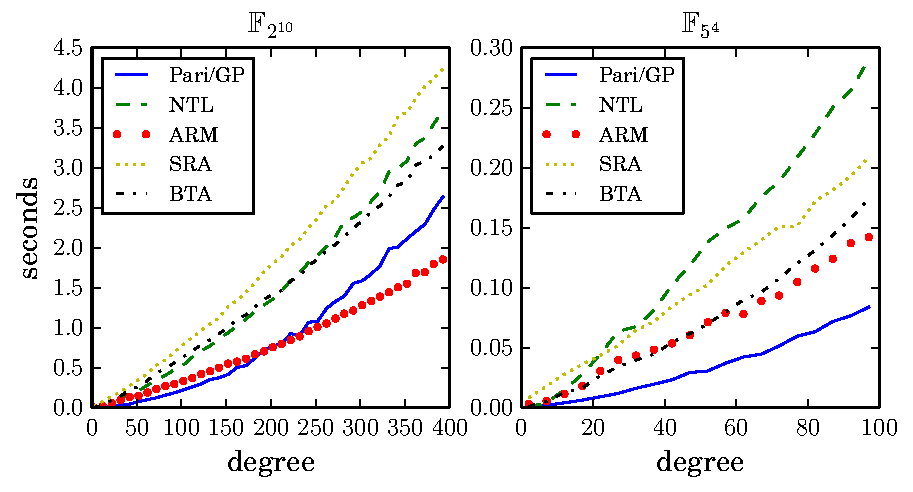
\includegraphics[width=0.55\textwidth]{benchmark}
  \caption{Timings in seconds for $\ff{2^{10}}$ (left) and $\ff{5^4}$
    (right). Abscissa is polynomial degree.}
  \label{fig:benchmarks}
\end{figure}

We used the versions of Pari/GP (v2.7.1) and NTL (v6.1.0) shipped in
the latest Sage distribution (v6.4.1). It should be noted that this is
not the latest NTL version, however we are not aware of any
performance improvements in the latest version (v8.0) concerning root
finding. It is also worth mentioning that the implementation of
polynomials over $\extf$ in Sage 6.4 is backed by the NTL library
(more precisely, by the multi-precision type \texttt{ZZ\_pEX}), thus
the performance of our implementation is essentially to be compared
with NTL's one.

To the best of our knowledge, both Pari/GP and NTL implement the
variant of Cantor-Zassenhaus~\cite{cantor1981} described
in~\cite{GathenS92}. The difference in performances is likely best
explained by the fact that the NTL type \texttt{ZZ\_pEX} is not the
best fit for small characteristic, while Pari/GP optimizes the field
element representation in this case. The fact that our own
implementations performed between the two, and sometimes even better,
shows that these algorithms are practical. However, the observed
differences in performance being so small, they are more likely
attributed to differences in the specific implementation, rather than
to the algorithms themselves.

We conclude that the algorithms reviewed in this paper are of
practical interest for finding polynomial roots in small
characteristic finite fields. In some cases, this in contrast with
what was previously thought, e.g., for ARM. Although general purpose
libraries will probably find no interest in implementing these
algorithms alongside the classical Cantor-Zassenhaus method, they may
turn out to have useful applications in particular finite field
problems.



\section{Conclusion and open problems}

computing $\alpha_i$ in $O(n)$

\paragraph{Aknowledgements} Luca De Feo would like to thank the
Pari/GP team for kindly hosting him in Bordeaux during the preparation
of the paper, and for giving him useful insights on the internals of
Pari/GP. He also thanks Jean-Pierre Flori for his invaluable help
figuring out the gory details of the Sage/NTL interface.

\bibliography{refs}
\bibliographystyle{plain}

\end{document}



% Local Variables:
% ispell-local-dictionary:"american"
% End:


%  LocalWords:  affine subspaces linearized factorizations
%  LocalWords:  iteratively
